% !TEX TS-program = xelatex
\documentclass[10pt,oneside,final]{article}

% Copyright 2017 Olivier Pieters 
% This document is licenses under GPL-3.0. View license.txt file for a copy of the license file. The figures in the /figures folder are licensed under the same license.
% Original GitHub repository: https://github.com/opieters/business-card

% set all margins to 0 and set business card size
\usepackage[paperwidth=2in,paperheight=3.5in,margin=0cm,noheadfoot]{geometry}
\setlength{\baselineskip}{0cm}
\setlength{\topskip}{0pt}

\usepackage{parskip}         % remove paragraph indents
\usepackage{fontspec}        % load external fonts
\usepackage{tikz}            % drawing
\usepackage{fontawesome}     % icon font
\usepackage{xcolor}          % more colour options
\usepackage{graphics}        % load images
\usepackage[nolinks]{qrcode} % create QR codes

% load and configure tikz libraries
\usetikzlibrary{matrix,calc,positioning}

% load external font
\setmainfont{Fira Sans}
\setsansfont{Fira Sans}
\setmonofont{Fira Mono}

% define some lengths for internal spacing
\newlength{\seplinewidth}    \setlength{\seplinewidth}{2cm}
\newlength{\seplineheight}   \setlength{\seplineheight}{1pt}
\newlength{\seplinedistance} \setlength{\seplinedistance}{0.2cm}

% colour options
\definecolor{seplinecolour}{HTML}{357f2d}  % green
\definecolor{iconcolour}{HTML}{2f3142}     % dark
\definecolor{textcolour}{HTML}{2f3142}     % dark
\definecolor{jobtitlecolour}{HTML}{474a65} % light dark

% define some lengths for internal spacing
\newlength{\qrheight}  \setlength{\qrheight}{1in}
\newlength{\edgemargin} \setlength{\edgemargin}{0.2in}
\newlength{\logowidth}  \setlength{\logowidth}{1in}

% define colours
\definecolor{bordercolour}{HTML}{357f2d} % green
\definecolor{backtextcolour}{HTML}{000000}   % black

% change global colour
\makeatletter
\newcommand{\globalcolor}[1]{%
  \color{#1}\global\let\default@color\current@color
}
\makeatother
\AtBeginDocument{\globalcolor{textcolour}}

% create additional icons
\tikzset{
  ic/.pic={
    \draw[rounded corners=#1/10,fill,black] (-5/10*#1,-5/10*#1) rectangle ++(10/10*#1,10/10*#1);
    \draw[rounded corners=#1/20,fill,black] (-4/10*#1,-4/10*#1) ++(#1/10,-#1/20) rectangle ++(#1/10,-2/10*#1);
    \draw[rounded corners=#1/20,fill,black] (-4/10*#1,-4/10*#1) ++(8/10*#1-#1/10,-#1/20) rectangle ++(-#1/10,-2/10*#1);
    \draw[rounded corners=#1/20,fill,black] (-4/10*#1,-4/10*#1) ++(#1/10,8/10*#1+#1/20) rectangle ++(#1/10,2/10*#1);
    \draw[rounded corners=#1/20,fill,black] (-4/10*#1,-4/10*#1) ++(8/10*#1-#1/10,8/10*#1+#1/20) rectangle ++(-#1/10,2/10*#1);
    \draw[rounded corners=#1/20,fill,black] (-4/10*#1,-4/10*#1) ++(8/10*#1+#1/20,#1/10) rectangle ++(2/10*#1,#1/10);
    \draw[rounded corners=#1/20,fill,black] (-4/10*#1,-4/10*#1) ++(8/10*#1+#1/20,8/10*#1-#1/10) rectangle ++(2/10*#1,-#1/10);
    \draw[rounded corners=#1/20,fill,black] (-4/10*#1,-4/10*#1) ++(-#1/20,#1/10) rectangle ++(-2/10*#1,#1/10);
    \draw[rounded corners=#1/20,fill,black] (-4/10*#1,-4/10*#1) ++(-#1/20,8/10*#1-#1/10) rectangle ++(-2/10*#1,-#1/10);
    \draw[rounded corners=#1/20,fill,white] (-3.5/10*#1,3.5/10*#1) circle (1/20*#1);
    \node[anchor=center,color=white] at (0,0) {\small IC};
  },
  ml/.pic={
    \draw[line width=1pt,inner color=gray,outer color=white] (0,0) circle (0.4/1.4);
    \draw[line width=0.75pt,line cap=round] ($(0,0)!1!50:(0,0.3/1.4)$) arc (140:-20:0.3/1.4);
    \draw[line width=0.5pt,line cap=round] ($(0,0)!1!30:(0,0.1/1.4)$) arc (120:0:0.1/1.4);
    \fill (0,0) circle (0.05/1.4);
  }
}

\begin{document}
  \thispagestyle{empty}
  %\vspace*{\fill}
  \begin{center}
    \begin{tikzpicture}
      % name
      \matrix[every node/.style={anchor=center,font=\huge},anchor=center] (name) {
        \node{Martin}; \\
        \node{Skarzynski}; \\
        %\node{\color{jobtitlecolour}\normalsize\textit{Cancer Prevention Fellow}}; \\
      };
      % sep line 1
      \node[below=\seplinedistance of name] (hl1) {};
      \draw[line width=\seplineheight,color=seplinecolour] (hl1)++(-\seplinewidth/2,0) -- ++(\seplinewidth,0);
      % contact info
      \matrix [below=\seplinedistance of hl1,%
               column 1/.style={anchor=center,color=iconcolour},%
               column 2/.style={anchor=west}] (contact){
        \node{\faGlobe}; & \node{marskar@github.io};\\
        \node{\faEnvelope}; &\node{marskar@gmail.com};\\
        \node{\faPhone}; &\node{+1 240 595 3460}; \\
        \node{\faLinkedin}; &\node{linkedin.com/in/mskar}; \\
        \node{\faTwitter}; &\node{twitter.com/marskar}; \\
        \node{\faGithub}; &\node{github.com/marskar}; \\
      };
      % sep line 2
      \node[below=\seplinedistance of contact] (hl2) {};
      \draw[line width=\seplineheight,color=seplinecolour] (hl2)++(-\seplinewidth/2,0) -- ++(\seplinewidth,0);
      % interests
      \matrix [below=\seplinedistance of hl2,
         every node/.style={anchor=center,font=\LARGE}]
         (interests) {
        \node{\faDatabase}; &
        \node{\faLineChart}; &
        \node{\faCode}; &
        \node{\faEdit}; &
        \node{\faSitemap}; \\
      }; 
    \end{tikzpicture}
  \end{center}
  \vspace*{\fill}
  
  \clearpage
  \globalcolor{backtextcolour}
  
  \thispagestyle{empty}
  \vspace*{\fill}
  \begin{tikzpicture}[remember picture,overlay,inner sep=0pt]
    \draw[fill=bordercolour!1,draw=bordercolour] (current page.center) ++(-\paperwidth/2+\edgemargin,\paperheight/2-\edgemargin) rectangle ++(\paperwidth-2*\edgemargin,-\paperheight+2*\edgemargin);
    % pic
    \draw (current page.center) ++(0,\paperheight/2-\edgemargin-\paperwidth/2+\edgemargin+\logowidth/2) node (helper logo) {};
    \node[anchor=north] at (helper logo) {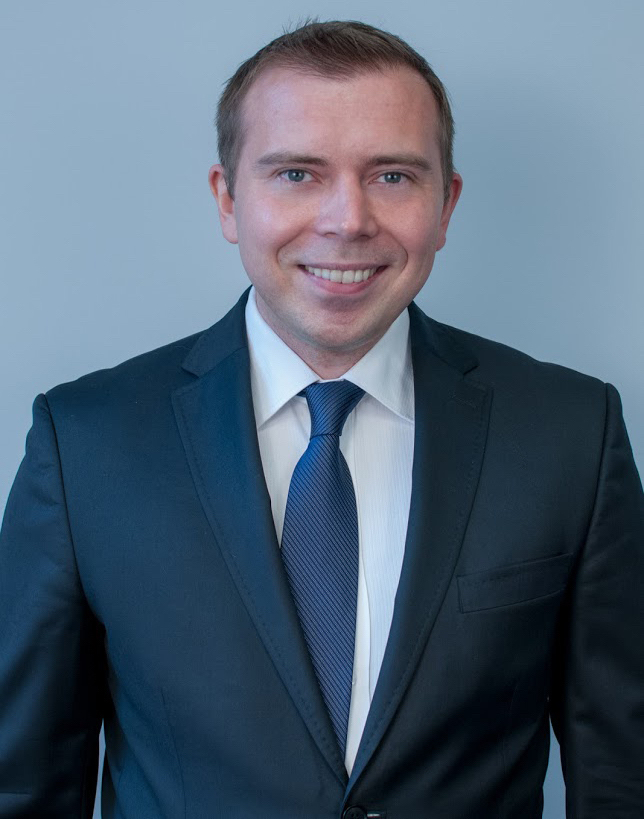
\includegraphics[width=\logowidth]{profpic.jpeg}};
    % qr code
\draw (current page.center) 
  ++(0,-\paperheight/2+\edgemargin+\paperwidth/2-\edgemargin-\qrheight/2) 
  node (helper qr) {};
\node[anchor=south] at (helper qr) 
  {\qrcode[level=M,height=\qrheight]{BEGIN:VCARD
VERSION:3.0
N:Martin;Skarzynski;;Dr.
FN:Dr. Martin Skarzynski
TITLE:Cancer Prevention Fellow
ORG:National Cancer Institute
%PHOTO;VALUE=URI;TYPE=JPEG:https://johndoe.com/path/to/jpeg/images.jpeg
TEL;TYPE=MOBILE:+1 240 595 3460
EMAIL:marskar@gmail.com
URL:https://marskar@github.io
REV:2017-29-01T13:52:43Z
%BDAY:19880310
%ADR;TYPE=WORK,PREF:;;2 Some Avenue;Anytown;SF;11111;USA
END:VCARD}};
  \end{tikzpicture}
  \vspace*{\fill}
  
\end{document}
